\section{Μη-Γραμμικός Ελεγκτής}

Στην αυτόνομη καθοδήγηση αιώρησης του αεροχήματος, οι συντεταγμένες \(x\) και 
\(y\) δεν αποτελούν αντικείμενο ενδιαφέροντος στο πλαίσιο της συγκεκριμένης 
εργασίας. Από το αφινικό σύστημα διαφαίνεται ότι οι μεταβλητές κατάστασης που 
απευθύνονται στις κινήσεις στους συγκεκριμένους άξονες, είναι αποσυμπλεγμένες 
από τις υπόλοιπες και μπορούν να απαλειφθούν από το σύστημα.

Σημειώνεται πως για την απλούστευση των εκφράσεων, πλέον, τα διανύσματα $(x_i), 
(y_i)$ κλπ θα συμβολίζονται απλώς ως $x, y$. 

Επιπλέον, πριν την αρχική σχεδίαση του μη-γραμμικού ελεγκτή γίνεται διαχωρισμός 
του δυναμικού συστήματος αφινικής δομής σε δύο υποσυστήματα, με το πρώτο να 
περιέχει τις εξισώσεις κινητικής και κατ' επέκταση τις δράσεις ελέγχου, και το 
δεύτερο τις εξισώσεις κινηματικής. Εξάγεται λοιπόν η μορφή

\begin{gather}
    \dot{x} = f_{0}(x, y) + 
        \sum_{i}^{m}{d_{i}f_{i}}(x, y)
        \label{ctl:knt} \\
    \dot{y} = A(y)x
    \label{ctl:knm}   
\end{gather}
όπου  
\begin{equation}
    f_0:\mathbb{R}^{n} \times V \rightarrow \mathbb{R}^{n}
    ,\qquad
    f_{0} = \begin{pmatrix}
        g \\ 
        -I_{G}^{-1}(\omega \times I_{G}\omega)
    \end{pmatrix}
    \label{ctl:f0}
\end{equation}
$f_{i}:\mathbb{R}^{n} \times V \rightarrow \mathbb{R}^{n}$ λείες απεικονίσεις 
που συνθέτουν πίνακα
\begin{equation*}
    G =\left(f_1, \ldots, f_{m}\right) = 
    \begin{pmatrix}
        m^{-1}\left(R_{3,1}, \, R_{3,3}\right) & 0_{1\times 3}\\
        0_{3\times 2} & I_G^{-1}
    \end{pmatrix}
\end{equation*}
και την λεία απεικόνιση $A:V\rightarrow\mathcal{L}(\mathbb{R}^{n})$
\begin{equation*}
    A(y) = \begin{pmatrix}
        1 & 0_{1\times 3} \\
        0_{3\times 1} & R_{eul}
    \end{pmatrix}
\end{equation*}
με τις μεταβλητές
\begin{align*}
    x &= \left(v_{z} \quad \omega_{x} \quad \omega_{y} \quad \omega_{z}
    \right)^{\intercal} \in \mathbb{R}^n\\
    y &= \left(z_{E} \quad e^{\scriptscriptstyle \intercal}\right)^{\intercal} 
    \in V \\
    d &= \left(T_x \quad T_z \quad M_x \quad M_y \quad M_z\right)^{\intercal} 
    \in \euclr m ,
\end{align*}
ενώ $n = 4, m = 5$. 

Από το σύστημα παρατηρείται ότι το ανοιχτό σύνολο $V = \mathbb{R} \times (-\pi, 
\pi) \times (-\pi/2, \pi/2) \times (-\pi, \pi)$. Επίσης το $span\{f_{i}(x,y)\} = 
\mathbb{R}^{n}$ για κάθε $x\in \mathbb{R}^n, y \in V$, δηλαδή ο πίνακας $G$ 
είναι πλήρης τάξης-$n$ που σημαίνει ότι το διάνυσμα εισόδου μπορεί να παράξει 
όλο τον χώρο των μεταβλητών $x$. Ακόμη, $A(V)\subset GL(\mathbb{R}^n)$, 
δηλαδή η $A(y)$ είναι αυτομορφισμός για κάθε $y\in V$.


Σταθεροποιούμε τυχόντα $x \in \mathbb{R}^n$ και $y\in V$, θέτουμε την 
γραμμική απεικόνιση 
\begin{equation*}
    \Lambda:\mathbb{R}^{m} \rightarrow \mathbb{R}^{n}, \quad \mathbb{R}^m \ni 
    d \mapsto \sum_{i}^{m}{d_{i}f_{i}}(x, y) \in \mathbb{R}^{n}.
\end{equation*}

Από το γεγονός ότι $span\{f_{i}(x,y)\} = \mathbb{R}^{n}$, λαμβάνουμε ότι
\begin{equation*}
    \dim{\ker{\Lambda^{\ast}}} = n - \dim{im{\Lambda^{\ast}}} = n - \dim{im
    {\Lambda}} = 0,
\end{equation*}
δηλαδή $\Lambda^{\ast}$ είναι ενριπτική (απο \ref{kern}). 

Από την ισότητα $\langle \Lambda^{\ast}x, \Lambda^{\ast}x \rangle = \langle 
(\Lambda \circ \Lambda^{\ast}) x, x\rangle$ συνεπάγεται ότι $\ker \Lambda 
\circ \Lambda^{\ast} = \{0\}$ και άρα η $\Lambda \circ \Lambda^{\ast}$ 
αυτομορφισμός. (Βλ. \ref{nlt_trm})

Το σύνολο λύσεων $S$ για σύστημα $\Lambda x = z$ με $z \in \mathbb{R}^n$ είναι 
\begin{equation*}
    S = \left\{x\in \mathbb{R}^m \, | \, \Lambda x = z\right\} = \left\{x_{0} + 
        x \, | \, x \in \ker{\Lambda},\, \Lambda x_{0} = z \right\}. 
\end{equation*}Βλ. \ref{lemma_sum}.

Μία λύση $x_0$ αποτελεί η 
\begin{equation*}
    x_0 = \left(\Lambda^{\ast} \circ \left(\Lambda \circ \Lambda^{\ast} \right)^
        {-1} \right)z
\end{equation*}
έτσι ώστε
\begin{equation*}
    \Lambda x_0 = z \Rightarrow \Lambda \circ \left(\Lambda^{\ast} \circ \left
    (\Lambda \circ \Lambda^{\ast} \right)^{-1} \right)z = z \Rightarrow z = z.
\end{equation*}

Επιπλέον η λύση $x_0$ αποτελεί στοιχείο του $S$ με ελάχιστη νόρμα. Πράγματι 
έχουμε ότι $x_0 \in im\Lambda^{\ast} = \ker{\Lambda}^{\perp}$ (απο \ref{dim}). 
Επίσης, αν $x_1 \in S$ με $x_1 \neq x_0$ τότε $\left(x_1 - x_0\right) \in 
\ker{\Lambda}$. Συνεπώς από Πυθαγόρειο Θεώρημα προκύπτει ότι 
\begin{equation*}
    \|x_1\|^2 = \|(x_1 - x_0) + x_0\|^2 = \|x_1 - x_0\|^2 + \|x_0\|^2 > \|x_0\|
    ^2.
\end{equation*}
 
Η απεικόνιση $\left(x, y\right) \mapsto \Lambda^{\ast} \circ \left(\Lambda \circ
\Lambda^{\ast} \right)^{-1}$ του $\mathbb{R}^{n} \times V$ στο $\mathcal{L}
(\mathbb{R}^{n}, \mathbb(R)^{m})$ είναι λεία και συμπεραίνεται από τον ακόλουθο 
συλλογισμό: Έστω $B$, η απεικόνιση, που αντιστοιχίζει σε κάθε $(x_{i})_1^{m} 
\in 
(\mathbb{R}^{n})^{m}$ την γραμμική απεικόνιση $(u_i)_1^{m} \mapsto 
\sum{u_{i}x_{i}}$. Η $B$ είναι ισομορφισμός του $(\mathbb{R}^{n})^{m}$ επί του 
$\mathcal{L}(\mathbb{R}^{n}, \mathbb{R}^{m})$ και άρα η $(x, y) \mapsto \Lambda$
είναι λεία, διότι είναι σύνθεση της $B$ με την απεικόνιση $\left(x, y\right) 
\mapsto \left(f_1(x, y), \ldots f_m(x, y) \right)$ η οποία είναι λεία διότι, 
όπως αναφέρθηκε, οι $f_i$ είναι λείες. Επιπρόσθετα, η $\Lambda \mapsto \Lambda
^{\ast}$ είναι γραμμική, άρα είναι λεία και το ίδιο ισχύει για τη σύνθεση 
γραμμικών απεικονίσεων $\left(A, B\right) \mapsto A\circ B$. Επειδή και η 
απεικόνιση $A \mapsto A^{-1}$ του $GL\left(\mathbb{R}^n\right)$ επί του 
$GL\left(\mathbb{R}^n\right)$ είναι λεία, καταλήγουμε, λοιπόν, ότι η $(x,y) 
\mapsto \Lambda^{\ast} \circ \left(\Lambda \circ \Lambda^{\ast} \right)^{-1}$ 
είναι λεία ως σύνθεση λείων απεικονίσεων.
% 3ο βήμα
Υποθέτουμε λεία απεικόνιση $\overline{v}:\mathbb{R}\times\mathbb{R}^n\times V 
\rightarrow \mathbb{R}^n$ και θέτουμε τις απεικονίσεις:
\begin{align*}
    % \overline{v}&:\mathbb{R}\times\mathbb{R}^n\times V \rightarrow \mathbb{R}^n,
    % \, \text{λεία} \\
    w&: \mathbb{R}^{n} \times V \rightarrow \mathcal{L}(\mathbb{R}^{n}, 
    \mathbb{R}^{m}),\quad (x, y) \mapsto \Lambda^{\ast} \circ 
    (\Lambda \circ \Lambda^{\ast})^{-1},\\
    d_{i}&:\mathbb{R} \times \mathbb{R}^{n} \times V \rightarrow \mathbb{R} 
        ,\quad d_{i}(t, x, y) = \pi_i\left((w(x,y))(\overline{v}(t,x,y)) 
        \right) \quad \text{για} \quad i \in \{1, \ldots, m\}.
\end{align*}
Κάθε προβολή $\pi_{i}$ είναι λεία απεικόνιση και το ίδιο ισχύει για την 
απεικόνιση $\left(A, x\right) \mapsto Ax$ του $\mathcal{L}\left(\mathbb{R}^{n}, 
\mathbb{R}^{m}\right) \times \mathbb{R}^{n}$ στο $\mathbb{R}^{m}$, γιατί είναι 
διγραμμική. Επομένως, κάθε $d_{i}$ είναι λεία απεικόνιση ως σύνθεση λείων 
απεικονίσεων. Αντικαθιστώντας προκύπτει ότι
\begin{gather*}
    \sum{d_i(t,x,y)f_i(x,y)}=\sum{\pi_{i}\left((w(x,y))(\overline{v}(t,x,y))
    \right) f_i(x,y)} = \Lambda \left( (w(x,y)) \overline{v}(t,x,y)\right) = \\ 
    = \Lambda\left(\left(\Lambda^{\ast} \circ (\Lambda \circ 
        \Lambda^{\ast})^{-1}\right) \overline{v}(t,x,y)\right) = 
        \overline{v}(t,x,y).
\end{gather*}

Θέτοντας μια ακόμη λεία απεικόνιση $v:\mathbb{R}\times\mathbb
{R}^n\times V \rightarrow \mathbb{R}^n $ κι αν $\overline{v}(t,x,y) = -f_0(x,y) 
+ v(t,x,y)$ το σύστημα (\ref{ctl:knt},\ref{ctl:knm}) μετασχηματίζεται σε
\begin{gather}
    \dot{x} = v(t,x,y)\\
    {\dot{y}} = A({y}) {x}.
\end{gather}
Έτσι, καταφέρνουμε να απορρίπτουμε το μη-γραμμικό διανυσματικό πεδίο $f_0$  από 
τις κινητικές εξισώσεις για κάθε $x,y$. Αυτό στη βιβλιογραφία αναφέρεται ως 
γραμμικοποίηση με ανάδραση (\tl{feedback linearization}).

Αντικείμενο του ελέγχου είναι η ακολούθηση μιας τροχιάς αναφοράς από τις 
μεταβλητές εξόδου $y$. Ορίζεται η δύο φορές συνεχώς διαφορίσιμη απεικόνιση 
$y_r:\mathbb{R}\rightarrow V$, η οποία αποτελεί το σήμα αναφοράς των μεταβλητών 
$y$. Ορίζεται επιπλέον η απεικόνιση $\alpha:\mathbb{R}\times V\rightarrow 
\mathbb{R}^n$ με $\alpha(t,y) = K_1(y-y_r(t)) + \dot{y}_r(t)$, όπου $K_1 \in 
\mathcal{L}(\mathbb{R}^n)$ γραμμικός μετασχηματισμός με ιδιοτιμές το αρνητικό 
ημιεπίπεδο. Η $\alpha$ είναι λεία ώς σύνθεση λείων απεικονίσεων. Έαν ταυτιστεί 
το διάνυσμα $\dot{y}$ με την απεικόνιση $\alpha$ τότε θα έχουμε
\begin{equation*}
    \dot{y} = a(t,y) \Rightarrow \dot{y} = K_1\left(y-y_r(t)\right) + 
    \dot{y}_r(t) \Rightarrow \dot{y} - \dot{y}_r(t) = K_1(y - y_r(t)),
\end{equation*}
θέτοντας τη μεταβλητή απόκλισης $\widetilde{y}:\mathbb{R}\times \mathbb{R}^n 
\rightarrow \mathbb{R}^n$ με $\widetilde{y} = y - y_r(t)$ παίρνουμε τη 
διαφορική εξίσωσης πρώτης τάξης $\dot{\widetilde{y}} = K_1 \widetilde{y}$, λύση 
της οποίας είναι $\widetilde{y} = e^{tK_1}\widetilde{y}_0 $ δηλαδή η μεταβλητή 
απόκλισης $\widetilde{y}$ τείνει εκθετικά στο 0 και ταυτόχρονα η μεταβλητή 
εξόδου $y$ τείνει στο σήμα αναφοράς $y_r$. Όμως, η δράση ελέγχου δε δρα 
απευθείας στις μεταβλητές εξόδου αλλά μέσω των μεταβλητών $x$.

Θέτουμε $f:\!GL\left(\mathbb{R}^n\right)\!\rightarrow GL\left(\mathbb{R}^n
\right)$ με $f\left(A\right)\!=\! A^{-1}$ και $\phi\!:\mathbb{R}\!\rightarrow 
\mathbb{R}^n$ με $\phi(t)\!= \left(\left(f \circ A\right)\left(y\left(t\right)
\right)\right)\alpha\left(t\right)$.

Όπως δείξαμε στην πρόταση (\ref{ctl:sen3}) για την απεικόνιση $\phi(t)$ θα 
ισχύει ότι
\begin{gather*}
    \dot{\phi} = \left(\left(f \circ A\right)(y)\right)'\alpha+ \left(\left(f 
    \circ A\right)(y)\right)\dot{\alpha} = \left(f'\left(A(y)\right)\left(A'(y)
    \dot{y}\right)\right)\alpha+ \left(\left(f \circ A\right)(y)\right)
    \dot{\alpha}\\
    = -\left(A(y)^{-1} \circ \left(A'(y)\dot{y}\right)\right) \left(A(y)^{-1} 
    \alpha \right) + A(y)^{-1}\dot{\alpha}  \\
    \text{που συνεπάγεται ότι }\quad\dot{\phi} = -\left(A(y)^{-1} \circ 
    \left(A'(y) \dot{y}\right)\right)\phi + A(y)^{-1}\dot{\alpha}.
\end{gather*}

Η ταύτιση $\dot{y} = \alpha$ ισοδυναμεί με $x = A(y)^{-1}a$. Παραγωγίζοντας 
παίρνουμε 
\begin{equation}
    \dot{x} = A(y)^{-1}\left(\dot{\alpha} - A'(y)\dot{y}x\right).
\label{x_dot}
\end{equation} 
% Όμως, η ολοκληρωτική καμπύλη  
Έτσι, η απεικόνιση $\theta$ είναι η ολοκληρωτική καμπύλη του λείου διανυσματικού 
πεδίου 
\begin{equation*}
    \mathbb{R} \times \mathbb{R}^n \ni(t,x) \mapsto A\left(y(t)\right)^{-1}
    \left(\dot{\alpha}(t) - A'\left(y(t)\right)\dot{y}(t)x\right) \in 
    \mathbb{R}^n
\end{equation*}
το οποίο για τυχαίο $t_0 \in \mathbb{R}$ διέρχεται από το $(t_0,A
\left(y(t_0)\right)^{-1}\alpha(t_0))$. Καθώς οι δράσεις ελέγχου ασκούνται στις
μεταβλητές $\dot x$, πρέπει να κατασκευαστεί μια έκφραση για τις $\dot x$ η 
οποία θα οδηγεί την $x$ στο $A(y)^{-1}a$. Όπως δείξαμε, δεν αρκεί απλώς να 
ικανοποιηθεί η σχέση (\ref{x_dot}) καθώς η ολοκληρωτική καμπύλη $\theta$ 
καθορίζεται από τις αρχικές συνθήκες.

Επιλέγεται ένας $K_2 \in \mathcal{L}(\mathbb{R}^n)$ με όλες τις ιδιοτιμές 
του $K_2$ να βρίσκονται στο αριστερό ημιεπίπεδο. Θέτουμε $b:\mathbb{R}\times
\mathbb{R}^n\times\mathbb{R}^n \rightarrow \realf^n$ με $b(t,x,\phi) = K_2(x - 
\phi(t))+\dot{\phi}(t)$. Εάν $\dot{x} = b$ τότε θα έχουμε
\begin{gather*}
    \dot{x} = b(t,x,\phi) = K_2(x - \phi(t))+\dot{\phi}(t), \quad
    \text{που συνεπάγεται}\quad \dot{x} - \dot{\phi}(t) = K_2(x - \phi(t)).
\end{gather*}
Έτσι, θέτοντας την μεταβλητή απόκλισης $\widetilde{x}:\mathbb{R}\times 
\mathbb{R}^n \rightarrow \mathbb{R}^n$ με $\widetilde{x} = x - \phi(t)$. 
Παίρνουμε λοιπόν $\dot{\widetilde{x}} = K_2 \widetilde{x}$, η λύση της οποίας 
είναι η $\widetilde{x}(t) = e^{tK_2} \widetilde{x}_0$ η οποία τείνει εκθετικά 
την μεταβλητή απόκλισης $ \widetilde{x}$ στο 0. Έτσι επιλέγεται $v(t,x,y) = 
b(t,x,\phi)$ δηλαδή ότι
\begin{equation}
    \begin{gathered}
        \overline{v}(t,x,y) = -f_0(x,y) + b(t,x,\phi) \\
        \text{ή ισοδύναμα} \\
        \overline{v}(t,x,y) = -f_0(x,y) + A(y)^{-1}(\dot{\alpha}(t) - 
        (A'(y)(A(y)x))A(y)^{-1}a(t)) + K_2(x - A(y)^{-1}a(t)).
    \end{gathered} \label{ctl:ctl}
\end{equation}

Με την εισαγωγή του όρου $K_2(x - A(y)^{-1}a(t))$ επιτυγχάνεται η σύγκλιση του 
όρου $x$ στο $A(y)^{-1}a$ ανεξαρτήτων αρχικών συνθηκών. Με τη σειρά τους και οι 
μεταβλητές εξόδου $y$ συγκλίνουν στο επιθυμητό σήμα.

\subsection{Στάθμιση Ελεγκτή}
\noindentΟι παράμετροι στάθμισης σε αυτόν τον ελεγκτή είναι τα μητρώα 
$K_1, K_2$ τα οποία επιλέγονται να είναι διαγώνια. Έτσι, οι ιδιοτιμές των 
μητρώων αυτών είναι τα διαγώνια στοιχεία των. Η ιδιαιτερότητα του συστήματος 
μας είναι ότι η σύγκλιση των μεταβλητών εξόδου $y$ στο σήμα αναφοράς $y(t)$ 
περνάει μέσα από τη σύγκλιση των μεταβλητών $x$ στη συνάρτηση $\phi(t)$. Η 
διαδικασία στάθμισης των μητρώων που θα ακολουθήσει έχει ως εξής, θεωρώντας την 
σύγκλιση των $x$ ακαριαία, θέτουμε τις επιθυμητές σταθερές χρόνου για τις 
μεταβλητές εξόδου. Στη συνέχεια επιλέγονται και οι ιδιοτιμές του μητρώου $K_2$ 
, ούτως ώστε να ικανοποιούνται οι φυσικοί περιορισμοί των ενεργοποιητών. Οι 
φυσικοί περιορισμοί προκύπτουν από τις προδιαγραφές των κατασκευαστών.

\textbf{Στάθμιση $K_1$} Το μητρώο $K_1 = -diag(\nicefrac{1}{\tau_z}, 
\nicefrac{1}{\tau_\phi},\nicefrac{1}{\tau_\theta},\nicefrac{1}{\tau_\psi})$ όπου
$\tau_i$ η σταθερά χρόνου σε απόκριση βηματικής μεταβολής συστήματος πρώτης 
τάξης για $i \in \{z, \phi, \theta, \psi\}$. Η σταθερά χρόνου ισοδυναμεί με το 
χρόνο που απαιτείται απο ένα σύστημα πρώτης τάξης να φθάσει στο $63,2 \%$ της 
τιμής αναφοράς. Για την μετατόπιση $z$ επιλέγεται μια σταθερά χρόνου 
$\tau_z = 0.15s$, για την γωνία $\phi\,(roll)$ επιλέγεται $\tau_\phi = 0.15s$,
για την γωνία $\theta\,(pitch)$ επιλέγεται $\tau_\theta = 0.15s$ και για την 
γωνία $yaw \psi$ επιλέγεται $\tau_\psi = 0.33s$. Το μητρώο που προκύπτει είναι 
\begin{equation*}
    K_1 = -
    \begin{pmatrix}
        6.67 & 0    & 0    & 0\\
        0    & 6.67 & 0    & 0\\
        0    & 0    & 6.67 & 0\\
        0    & 0    & 0    & 3
    \end{pmatrix}.
\end{equation*}

Η απόκριση σε βηματικές μεταβολές του διανύσματος εξόδου $y$ φαίνεται παρακάτω.
\begin{figure}[H]
    \centering
    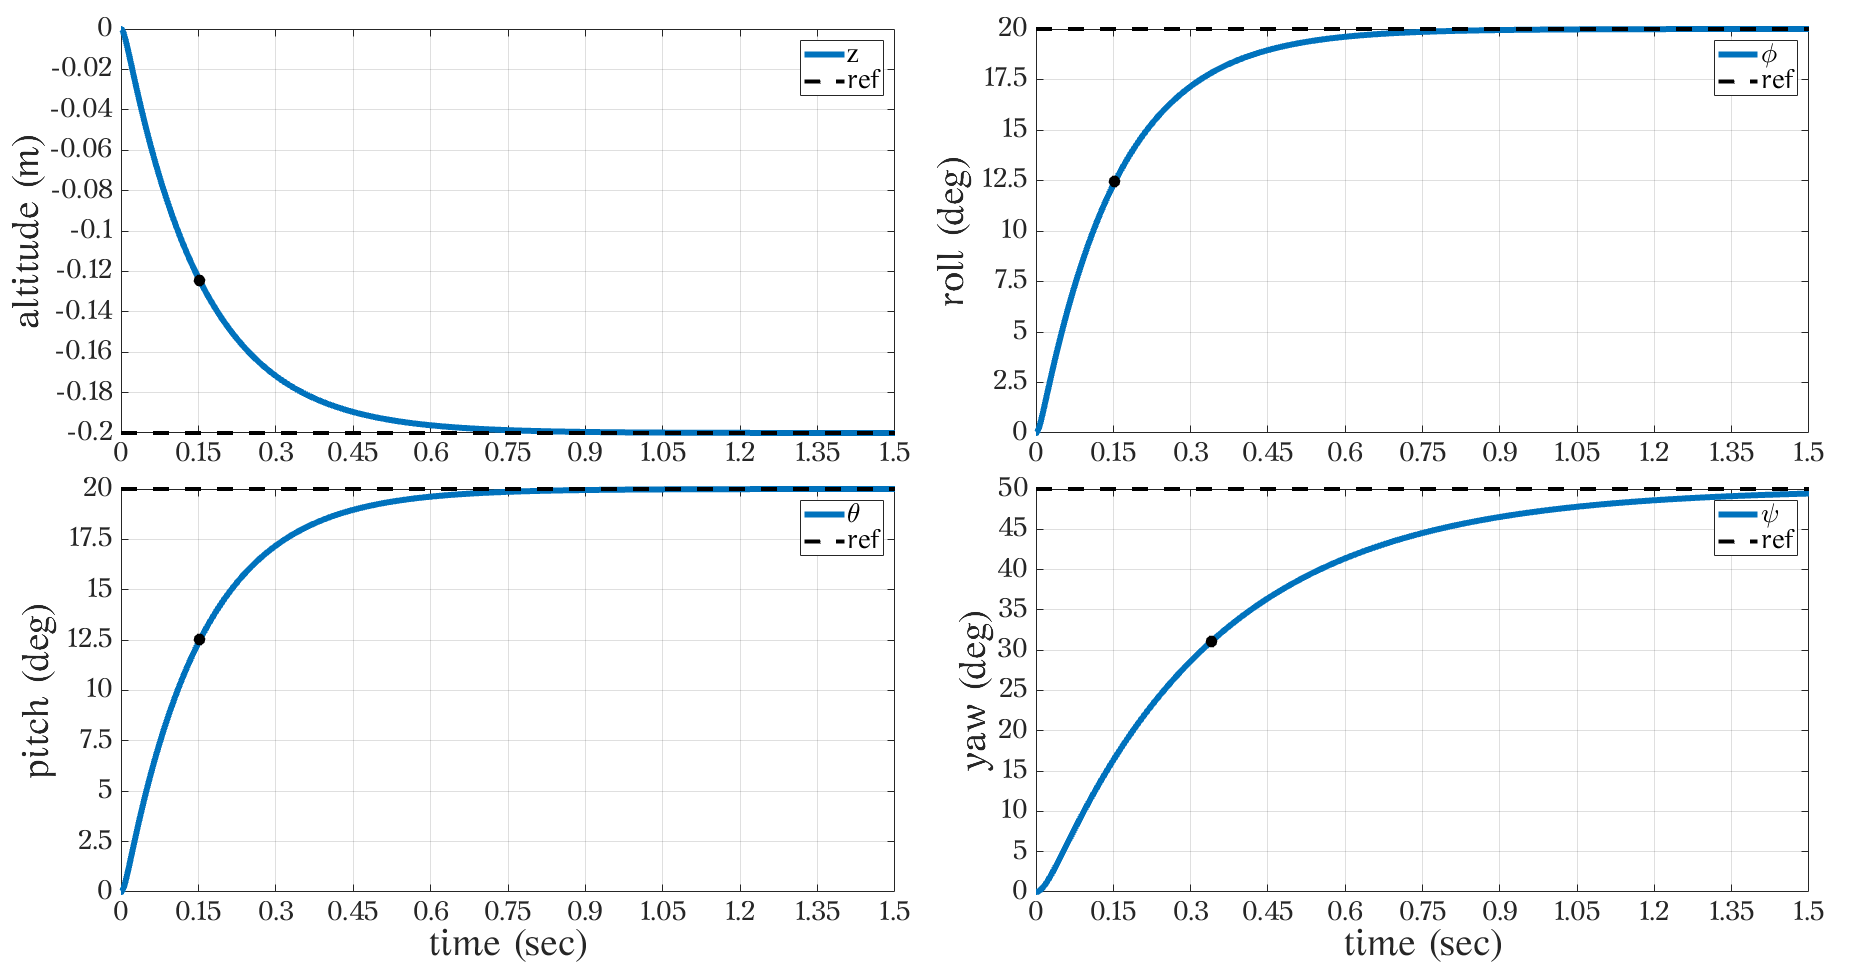
\includegraphics[width=1\textwidth]{Control/Nominal/fig_testeig.png}
    \caption{Βηματικές μεταβολές μεταβλητών εξόδου.}\label{fig:testig}
\end{figure}
Στα άνωθεν διαγράμματα σημειώνεται με μαύρη βούλα το σημείο όπου πετυχαίνουμε 
την επιθυμητή σταθερά χρόνου. Ενδεικτικά για το διάγραμμα του ύψους $z$, η βούλα
βρίσκεται στο σημείο $t = 0.15s$ και $z = -0.1247m$ δηλαδή στο $\frac
{-0.1247}{-0.20} = 62.35 \%$. (Σημείωση: η $z$ διεύθυνση στο αδρανειακό σύστημα 
αναφοράς είναι στραμμένη προς το κέντρο της γης, δηλαδή η βηματική μεταβολή του
γραφήματος αντιπροσωπεύει μια αύξηση του ύψους του τρικοπτέρου κατά 20 $\si{cm}$.)
Οι τιμές που απαιτήθηκαν για το διάνυσμα εξόδου είναι αντιπροσωπευτικές για 
τη λειτουργία του τρικόπτερου με την έννοια ότι είναι ρεαλιστικές τιμές που 
μπορεί να ζητηθούν από μια καμπύλη σήματος αναφοράς ανάμεσα σε δύο διαδοχικούς 
χρόνους.

\textbf{Στάθμιση $K_2$} Η διαδικασία που προηγήθηκε θεωρούσε τα δυναμικά 
των μεταβλητών $x$ ακαριαία. Για να προσδιοριστούν τα στοιχεία του διαγώνιου 
μητρώου $K_2 = -diag(\nicefrac{1}{\tau_{v_z}}, \nicefrac{1}{\tau_{\dot{\phi}}},
\nicefrac{1}{\tau_{\dot{\theta}}},\nicefrac{1}{\tau_{\dot{\psi}}})$ θεωρούμε μια 
αρχική δομή του μητρώου ως $K_2 = -diag(\nicefrac{1}{0.1}, \nicefrac{1}{0.1},
\nicefrac{1}{0.1},\nicefrac{1}{0.3})$. Όπως φαίνεται η δομή αυτή ομοιάζει με τη
στάθμιση του μητρώου $K_1$ πράγμα λογικό αφού τα στοιχεία τους αναφέρονται στην
επίτευξη του ίδιου σκοπού. Δοκιμάζοντας την αρχική εικασία $K_2$ παρατηρήθηκε 
πως βρισκόμαστε κοντά στα όρια των ενεργοποιητών. Έτσι μετακινήθηκαν όλες οι 
ιδιοτιμές πλησιέστερα στο μηδέν. Η τελική μορφή του μητρώου $K_2$ είναι
\begin{equation*}
    K_2 = -
    \begin{pmatrix}
        8 & 0 & 0 & 0\\
        0 & 8 & 0 & 0\\
        0 & 0 & 8 & 0\\
        0 & 0 & 0 & 2.66
    \end{pmatrix}.
\end{equation*}

\subsection{Αποτελέσματα}
Παρακάτω παρουσιάζονται ορισμένα αποτελέσματα. Αρχικά, απαιτείται από τη γωνία 
$\phi$ να ακολουθήσει ένα ημιτονοειδές σήμα αναφοράς $\phi_r(t) = 0.349\cos(t)$ 
, δηλαδή εύρος $\ang{20}$ και συχνότητα $\nicefrac{1}{2\pi}\,Hz$. Όπως φαίνεται, 
οι αρχικές συνθήκες της γωνίας $\phi$ δεν συμπίπτουν με την τιμή $\phi_r(0)$ 
, πράγμα που αντιλαμβάνεται ο ελεγκτής και 'στέλνει' εκθετικά τη γωνία $\phi$ 
στο σήμα αναφοράς, όπως φαίνεται και στις αρχικές δράσεις ελέγχου.
\begin{figure}[H]
    \centering
    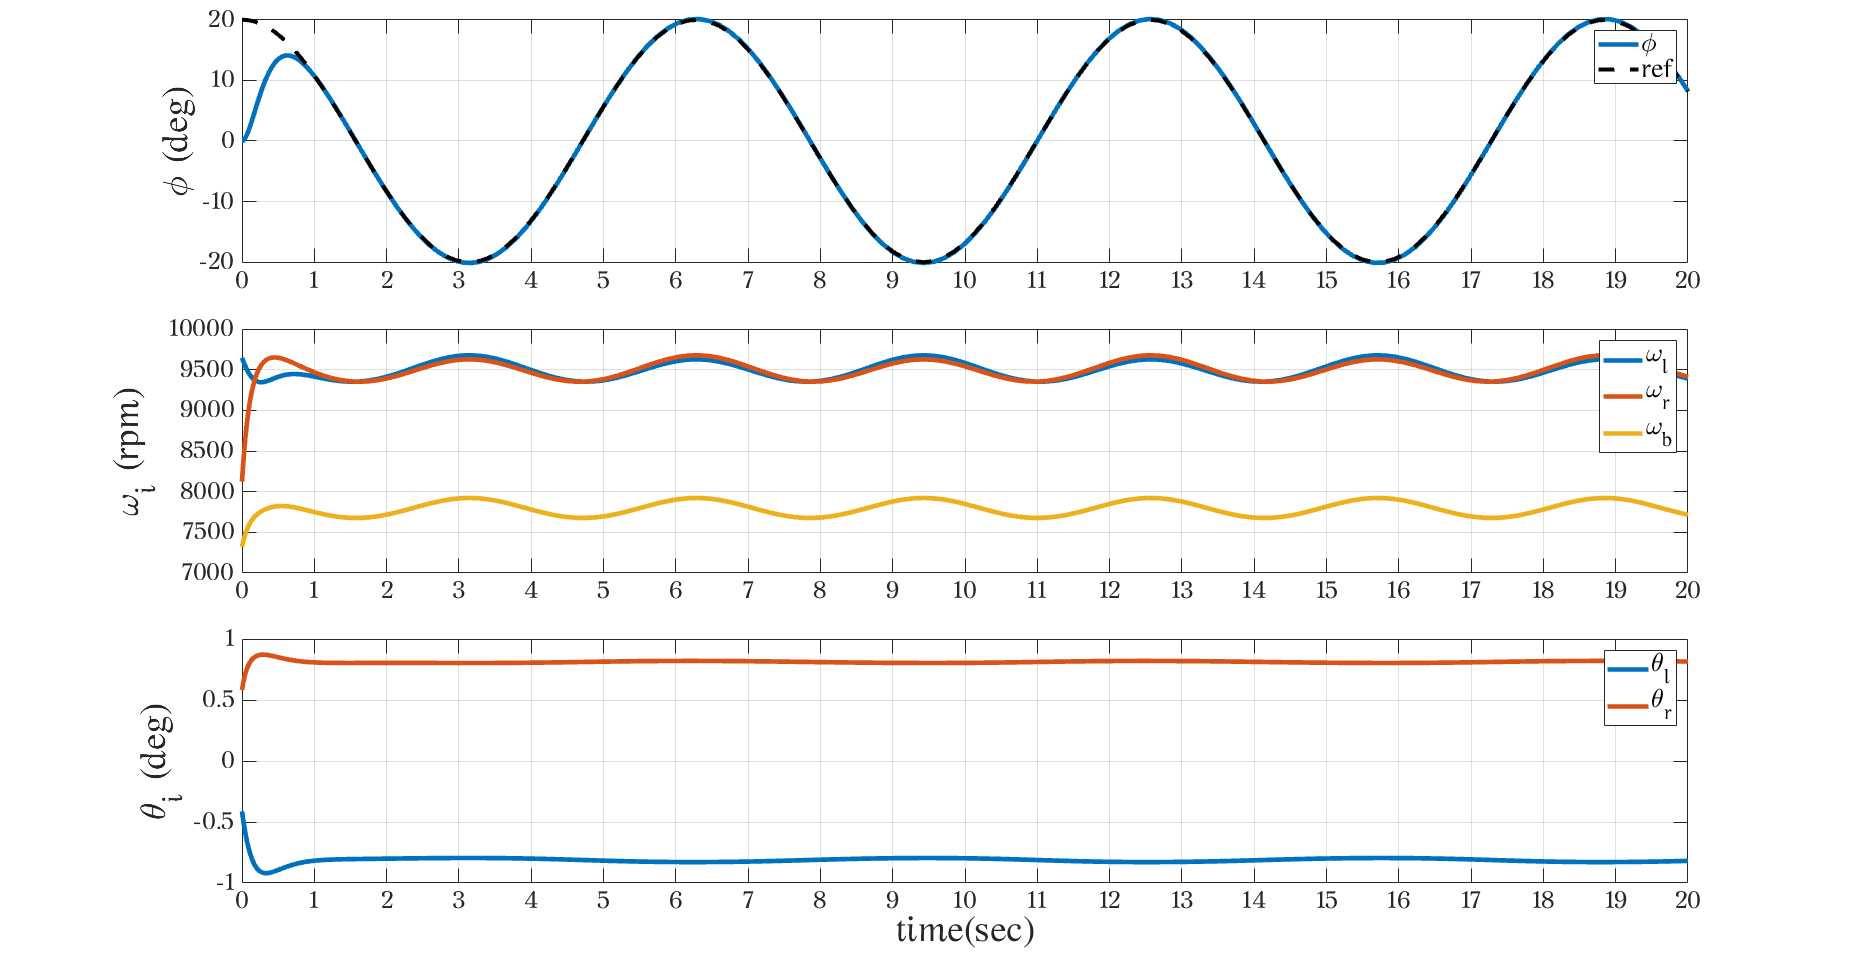
\includegraphics[width=1\textwidth]{Control/Nominal/fig_roll.png}
    \caption{Ακολούθηση σήματος αναφοράς γωνίας $\phi$.}\label{fig:roll}
\end{figure}

Στη συνέχεια ζητείται από το τρικόπτερο να ακολουθήσει ένα σήμα αναφοράς για τη 
γωνία $\theta$. Το σήμα αναφοράς είναι $\theta_r(t) = 0.349\cos(t/1.5)$ με 
εύρος $\ang{20}$ και συχνότητα $0,1\,Hz$. Τα αποτελέσματα για την γωνία 
$\theta$ παρουσιάζουν παρουσιάζουν αντίστοιχη σύγκλιση στο σήμα αναφοράς. 
\begin{figure}[H]
    \centering
    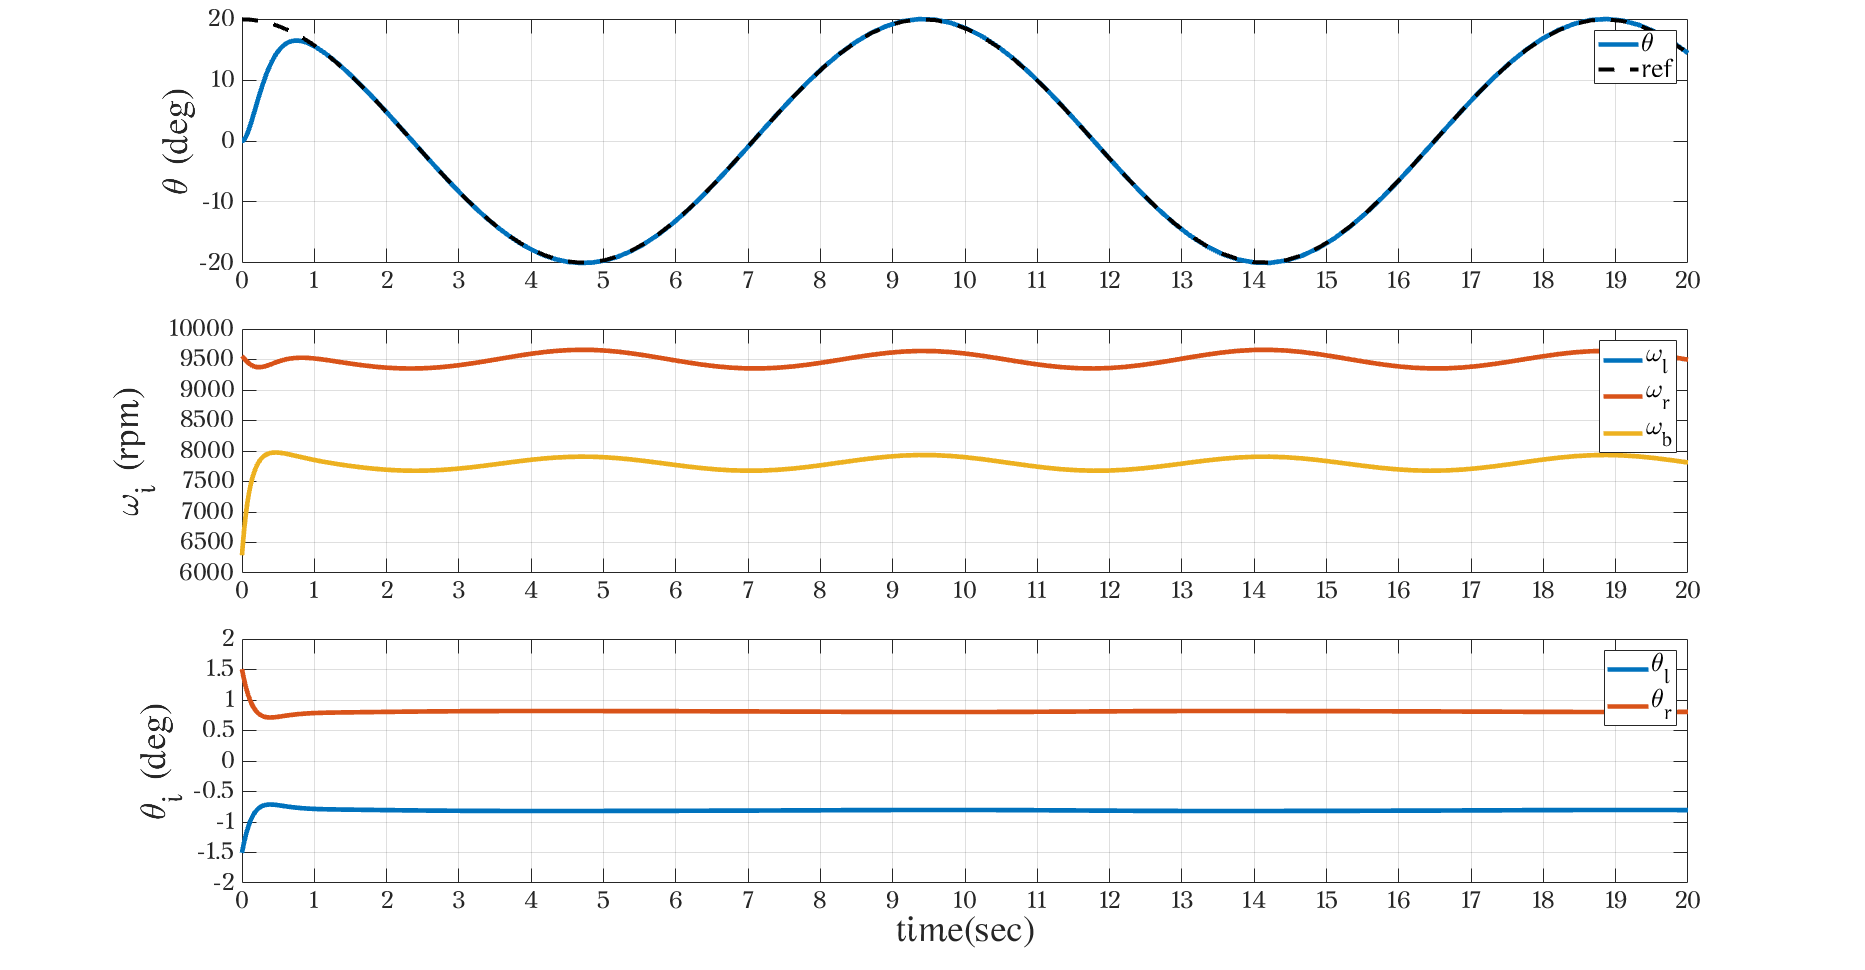
\includegraphics[width=1\textwidth]{Control/Nominal/fig_pitch.png}
    \caption{Ακολούθηση σήματος αναφοράς γωνίας $\theta$.}\label{fig:pitch}
\end{figure}

Ένα πιο ρεαλιστικό σενάριο πτήσης είναι αυτό που παρουσιάζεται παρακάτω. Η πτήση
ως τρικόπτερο χρησιμεύει κυρίως για την κάθετη απογείωση και την προετοιμασία
του αεροχήματος για την πτήση ώς αερόχημα σταθερής πτέρυγας. Έτσι, απαιτείται 
από το τρικόπτερο να ανυψωθεί ως ένα ύψος $30m$ σε χρόνο $10s$, ικανό για την 
μετάβαση σε συμβατική πτήση. Έπειτα, μόλις φθάσει σε αυτό το ύψος ζητείται από 
το τρικόπτερο να μεταβεί στον επιθυμητό προσανατολισμό (\tl{yaw}) που στην 
περίπτωση μας είναι $\ang{50}$ σχετικά με το Βορρά. Σε πραγματικές συνθήκες 
πτήσης είναι πιθανό, στην αρχική τοποθέτηση του αεροχήματος στο έδαφος, να 
υπάρχουν μη-μηδενικές αρχικές συνθήκες στις γωνίες. Στην περίπτωση που μελετάται
, το αερόχημα ξεκινάει από αρχικό προσανατολισμό $\left(\phi, \theta, 
\psi\right)_0 = \left(\ang{-20},\,\ang{20},\ang{-10}\right)$. Η καμπύλη που 
χρησιμοποιείται για το σήμα αναφοράς στο ύψος είναι η σιγμοειδής καμπύλη. Τα 
αποτελέσματα αυτού του σεναρίου παρουσιάζονται εδώ.
\begin{figure}[H]
    \centering
    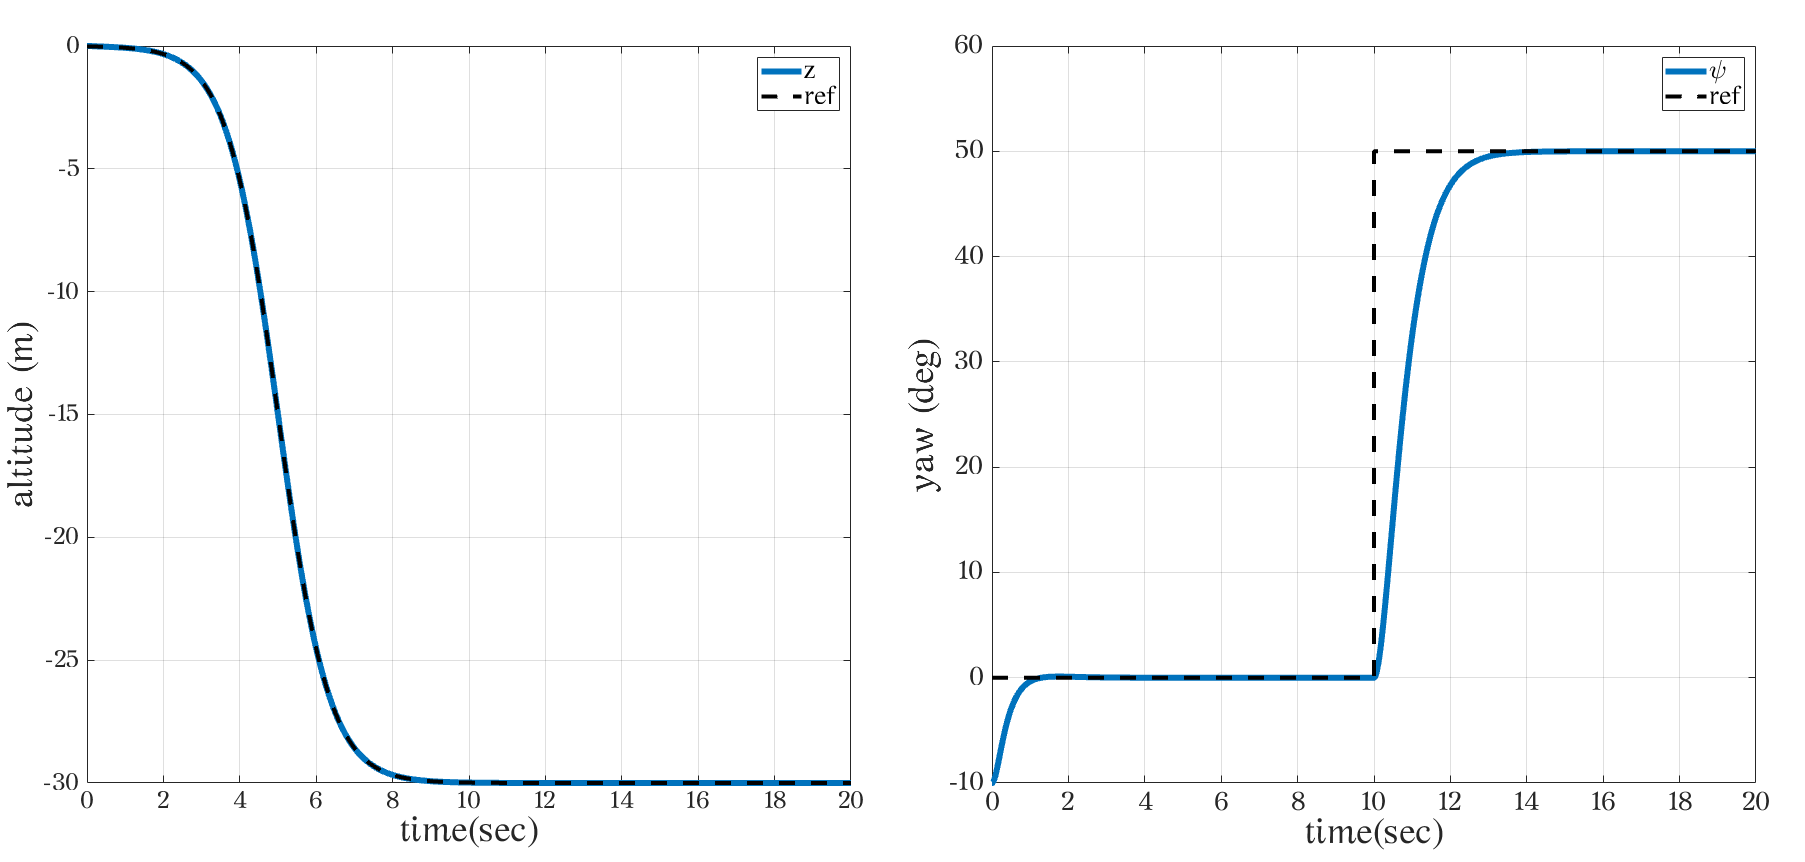
\includegraphics[width=1\textwidth]{Control/Nominal/fig_sigmoid_1.png}
    % \caption{Ακολούθηση σήματος αναφοράς γωνίας $\theta$.}\label{fig:pitch}
\end{figure}
\begin{figure}[H]
    \centering
    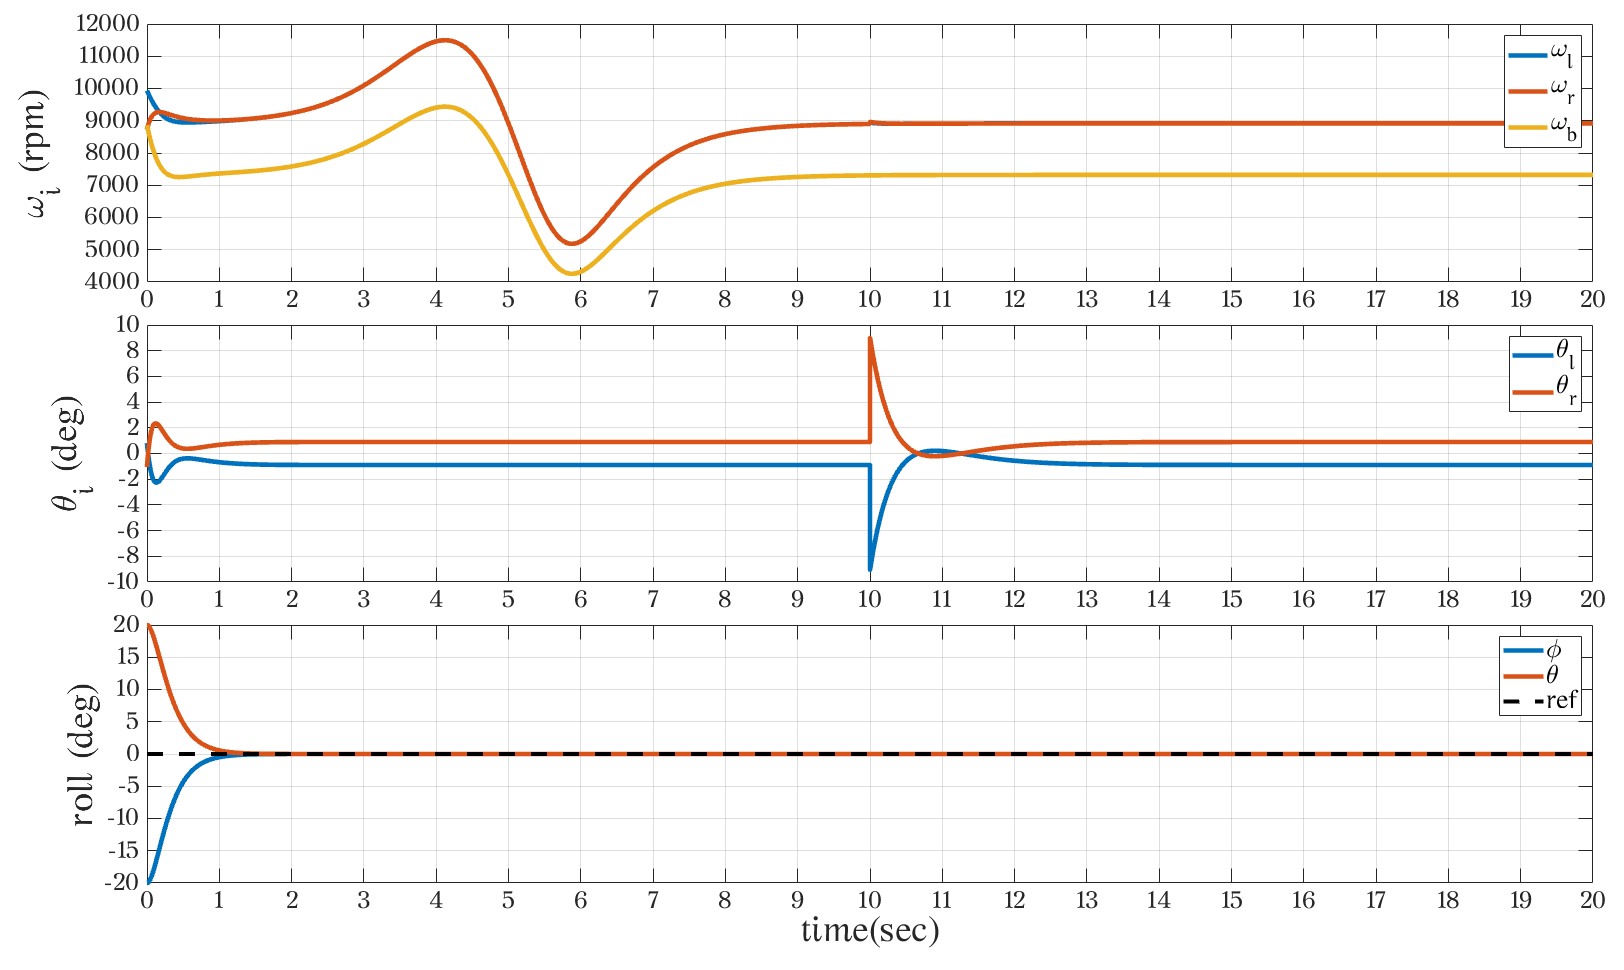
\includegraphics[width=1\textwidth]{Control/Nominal/fig_sigmoid_2.png}
    \caption{Απογείωση τρικοπτέρου σε συγκεκριμένο ύψος και επίτευξη επιθυμητού 
    προσανατολισμού.}\label{fig:takeoff}
\end{figure}

Παρατηρούμε, στα παραπάνω διαγράμματα, ότι ο ελεγκτής εκτελεί επιτυχώς το 
ζητούμενο σενάριο, χωρίς να εξωθούνται οι ενεργοποιητές να λειτουργήσουν στις 
μέγιστες επιτρεπόμενες τιμές τους. Συγκεκριμένα, η ακολούθηση της επιθυμητής 
τροχιάς του ύψους είναι απόλυτη, πράγμα που δικαιολογείται εν μέρει από την 
ταύτιση των αρχικών συνθηκών με το σήμα αναφοράς στο μηδενικό χρόνο.
